\documentclass[11pt]{article}
\usepackage[margin=1in]{geometry}
\usepackage{titlesec}
\usepackage{url}
\usepackage{hyperref}
\usepackage{amsmath}
\usepackage{enumitem} % in preamble
\usepackage{graphicx}
\graphicspath{{../Screenshots/}}
\setlist[itemize]{leftmargin=*, nosep, topsep=0pt, partopsep=0pt}

\newcommand{\memoheader}[4]{
  \noindent
  \textbf{From:} #2\\ 
  \textbf{To:} #1\\
  \textbf{Date:} #3\\
  \textbf{Subject:} #4\\[1ex]\hrule\vspace{1.5ex}
}

\begin{document}
\memoheader{Prof. Susan Gentry}
            {Miguel Cuaycong}
            {\today}
            {EMS 164: Simulation Memo 2}



\noindent The purpose of this memo is to present a simulation of interdiffusion which calculates the concentration of Gallium 
in an Fe/Fe-24Ga couple. Fe-24Ga is an alloy composed of Fe and Ga with 24 atomic\% of Ga. 
The parameters used and the simulation itself have are based on the experiment conducted in the paper "Composition dependence of tracer diffusion coefficients in Fe–Ga
alloys: A case study by a tracer-diffusion couple method"[1].
The primary mathematical model used is Fick's second law of diffusion of the form $\frac{dC_{Ga}}{dt} = D \frac{d^2c}{dx^2}$. 
The concentration surface $C_{Ga}(x,t)$ is evaluated using a numerical method called forward Euler.
Forward Euler has the form $C_{Ga}(x,t) = C_{Ga}(x, t-1) + \Delta t \frac{dC_{Ga}}{dt}$.
\\~\\
The parameters of the conducted experiment in the paper are the following: 
\begin{enumerate}
  \item 1143 K (below $\alpha-\gamma$ transition temperature and above the Curie point of pure Fe).
  \item 5 hours
  \item Pressure of $6(10)^{-3}$ Pa
\end{enumerate}
At this thermodynamic state, Fe-Ga has a BCC crystal structure according to the paper. This means atomistic diffusion will be due to jumps via vacancies instead of interstitially.
Bulk diffusion will occur due to the concentration gradient following Fick's second law. 
\\~\\
In the paper, the experiments can be classified to two kinds: tracer diffusion and interdiffusion. 
The experiment that is significant to this simulation is the interdiffusion experiment, particularly the Fe/Fe-24Ga couple.
Once the couple was allowed to interdiffuse for 5 hours, it is sectioned with a slow speed diamond saw and the diffusion profile measured in an EPMA.
Experimental results of this couple is shown in fig 5a of the paper.
\\~\\
The steps to the simulation is outlined as follows:
\begin{enumerate}
  \item Establish an initial concentration profile for Gallium in the calculation domain (-300 microns to 300 microns, increments of $\Delta x = 1 micron$). This is stored as the first element in a concentration matrix (t=0).
  \item Forward euler is then used to calculate the concentration profile for the next time step. Each step stored in the same concentration matrix. The inputs to the forward euler function are:
  \begin{enumerate}
    \item $\frac{d^2c}{dx^2}$
    \item $\Delta t$
    \item $D_{Ga} = 0.125 \frac{\text{microns}^2}{s}$
  \end{enumerate}
  \item $\frac{d^2c}{dx^2}$ will be recursively calculated for each concentration profile. 
\end{enumerate}
The simulation is robust enough to include or exclude the boundary condition of 
$C_{Ga} = 0$ for $x = [-300, 0]$, $C_{Ga} = 24$ for $x = [0, 300]$. These steps will produce a concentration matrix containing all concentration profiles for each time increment $\Delta t$.
\begin{figure}[!htbp]
    \centering
    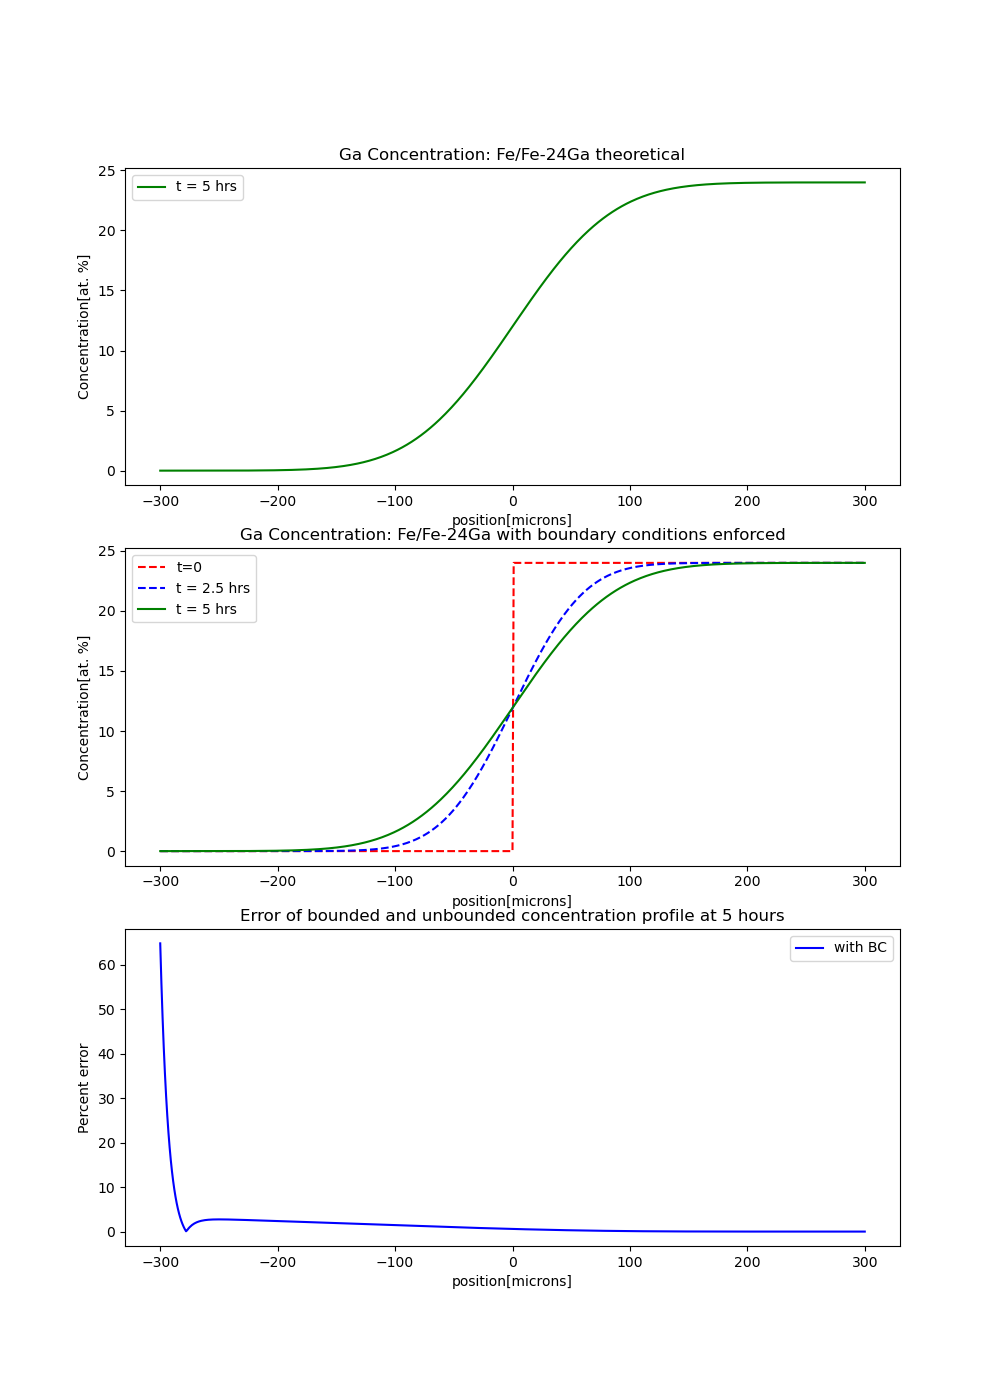
\includegraphics[width=350pt]{Ga_Concentration.png}
    \caption{(top) shows the theoretical concentration profile.
    (middle) shows the concentration profile of Ga with boundary conditions of $C_{Ga} = 2.4$ at $x = 300\,\mu m$ and $C_{Ga} = 0$ at $x = -300\,\mu m$.(bottom) Shows the error between the two concentration profiles at $t = 5$ hrs.}
    \label{fig:ga_profile}
\end{figure}
\\~\\
The function to produce the theoretical data is: $C(t,x) = \frac{C_{right} + C_{left}}{2} + \frac{C_{right} - C_{left}}{2}\text{erf}(\frac{x}{2\sqrt{Dt}})$
This is the solution to a couple which will be used to validate and compare the results of the forward euler prodiced matrix. The spike in error found in Fig 1. is due to the boundary condition forcing concentration to be 0 at x = -300
\section*{References}
[1] G.\ M.\ Muralikrishna, B.\ Tas, N.\ Esakkiraja, V.\ A.\ Esin, K.\ C.\ Hari\ Kumar, I.\ S.\ Golovin, I.\ V.\ Belova, G.\ E.\ Murch, A.\ Paul, and S.\ V.\ Divinski, ``Composition dependence of tracer diffusion coefficients in Fe--Ga alloys: A case study by a tracer-diffusion couple method,'' \textit{Acta Materialia}, vol.\ 203, Art.\ no.\ 116446, 2021, doi:\ 10.1016/j.actamat.2020.10.065.
\end{document}